\documentclass{article}
\usepackage[utf8]{inputenc}
\usepackage{graphicx}

\begin{document}

\section{Integration of Biometric Sensors with Arduino NANO-BLE33 and ESP-01}

\subsection{Hardware Configuration}
The biometric data collection system comprises the following hardware components:
\begin{itemize}
    \item \textbf{Arduino NANO-BLE33:} Central to the collection and initial processing of biometric data, including heart rate and galvanic skin response (GSR).
    \item \textbf{ESP-01:} Functions as a WiFi module, enabling the Arduino NANO-BLE33 to connect to the internet and transmit data using MQTT.
    \item \textbf{MAX30105 Heart Rate Sensor:} Connected to the Arduino for monitoring the user's heart rate.
    \item \textbf{GSR Sensor:} Attached to the Arduino for measuring galvanic skin response.
\end{itemize}
\subsection{Hardware Setup Diagram}
The following diagram illustrates the physical connections between the Arduino NANO-BLE33, ESP-01, and the biometric sensors (Heart-rate and GSR sensors).

\begin{figure}[h]
    \centering
    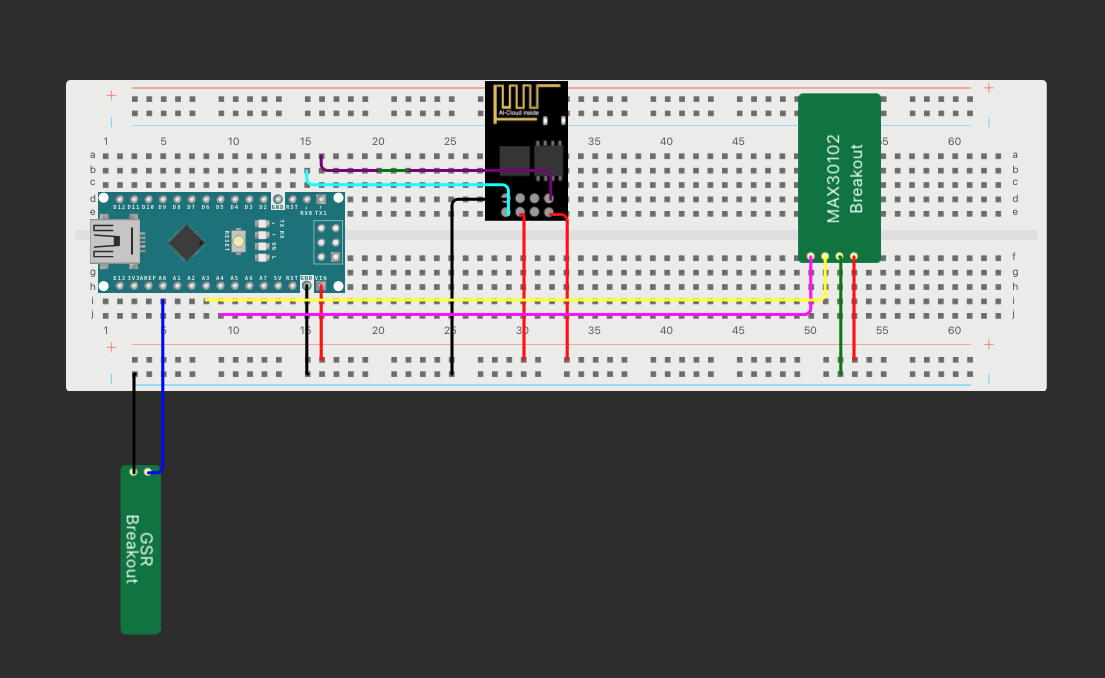
\includegraphics[width=0.8\textwidth]{../images/gsr&heart.png}
    \caption{Hardware connection diagram of Arduino NANO-BLE33 with ESP-01 and biometric sensors.}
    \label{fig:hardware-setup}
\end{figure}

\subsection{Arduino NANO-BLE33 Software Implementation}
The Arduino NANO-BLE33 is programmed to collect data from the heart rate and GSR sensors. Key aspects of the implementation include:
\begin{itemize}
    \item Initializing the MAX30105 sensor and configuring it for heart rate detection.
    \item Reading the GSR sensor data from the analog pin (A0).
    \item Calculating the beats per minute (BPM) and preparing a JSON payload.
    \item Sending the JSON payload to the ESP-01 via Serial communication.
\end{itemize}
\begin{verbatim}
#include <Wire.h>
#include "MAX30105.h"
#include "heartRate.h"
// .. ...
 String jsonPayload = "{\"SensorValue\":";
 jsonPayload += sensorValue;
 jsonPayload += ", \"BPM\":";
 jsonPayload += beatsPerMinute;
 jsonPayload += "}";

  Serial.println(jsonPayload);
\end{verbatim}

\subsection{ESP-01 Software Implementation}
The ESP-01 module is programmed to receive the biometric data from the Arduino NANO-BLE33 and publish it to an MQTT broker. The implementation covers:
\begin{itemize}
    \item Establishing a WiFi connection.
    \item Setting up MQTT client and handling reconnections.
    \item Reading data from the Arduino via Serial communication.
    \item Publishing the received data to the MQTT broker under the topic "sensor3/data".
\end{itemize}


\subsection{MQTT Communication Protocol}
The system utilizes MQTT for data transmission, offering a lightweight and reliable method to send sensor data to the central server. The ESP-01 acts as the MQTT publisher, transmitting data on the topic "sensor3/data". This setup ensures real-time data transfer with minimal bandwidth usage.

\subsection{Challenges and Solutions}
During the integration of the biometric sensors with the Arduino and ESP-01, several challenges were encountered and subsequently addressed:
\begin{itemize}
\item \textbf{Serial Communication:} The initial challenge was to establish a stable and reliable serial communication between the Arduino NANO-BLE33 and the ESP-01. This was achieved by setting a consistent baud rate and implementing a protocol to ensure complete data packets were sent and received.
\item \textbf{Data Parsing:} Parsing the JSON payload received from the Arduino on the ESP-01 posed a challenge due to variations in the data length. A robust parsing mechanism was developed to accurately extract BPM and GSR values from the payload.
\item \textbf{MQTT Connectivity:} Maintaining a stable MQTT connection, especially handling reconnections and network instability, was critical. This was addressed by implementing a reconnection strategy in the ESP-01’s software.
\end{itemize}

\subsection{Testing and Validation}
The system underwent extensive testing to validate its functionality. This included:
\begin{itemize}
\item Real-time monitoring of BPM and GSR data on the MQTT broker to ensure accurate and timely data transmission.
\item Stress-testing the system under various network conditions to validate the robustness of the MQTT reconnection mechanism.
\item Verifying the consistency and reliability of the data received from the sensors.
\end{itemize}

\subsection{Conclusion}
The integration of the Arduino NANO-BLE33 with the ESP-01 for biometric data collection and transmission via MQTT represents a significant advancement in the biometric verification system. This setup not only provides real-time data monitoring but also enhances the system's capability to handle biometric data efficiently.

\end{document}
